\documentclass[hidelinks,12pt]{article}
\usepackage[left=0.25cm,top=1cm,right=0.25cm,bottom=1cm]{geometry}
%\usepackage[landscape]{geometry}
\textwidth = 20cm
\hoffset = -1cm
\usepackage[utf8]{inputenc}
\usepackage[spanish,es-tabla]{babel}
\usepackage[autostyle,spanish=mexican]{csquotes}
\usepackage[tbtags]{amsmath}
\usepackage{nccmath}
\usepackage{amsthm}
\usepackage{amssymb}
\usepackage{mathrsfs}
\usepackage{graphicx}
\usepackage{subfig}
\usepackage{standalone}
\usepackage[outdir=./Imagenes/]{epstopdf}
\usepackage{siunitx}
\usepackage{physics}
\usepackage{color}
\usepackage{float}
\usepackage{hyperref}
\usepackage{multicol}
%\usepackage{milista}
\usepackage{anyfontsize}
\usepackage{anysize}
%\usepackage{enumerate}
\usepackage[shortlabels]{enumitem}
\usepackage{capt-of}
\usepackage{bm}
\usepackage{relsize}
\usepackage{placeins}
\usepackage{empheq}
\usepackage{cancel}
\usepackage{wrapfig}
\usepackage[flushleft]{threeparttable}
\usepackage{makecell}
\usepackage{fancyhdr}
\usepackage{tikz}
\usepackage{bigints}
\usepackage{scalerel}
\usepackage{pgfplots}
\usepackage{pdflscape}
\pgfplotsset{compat=1.16}
\spanishdecimal{.}
\renewcommand{\baselinestretch}{1.5} 
\renewcommand\labelenumii{\theenumi.{\arabic{enumii}})}
\newcommand{\ptilde}[1]{\ensuremath{{#1}^{\prime}}}
\newcommand{\stilde}[1]{\ensuremath{{#1}^{\prime \prime}}}
\newcommand{\ttilde}[1]{\ensuremath{{#1}^{\prime \prime \prime}}}
\newcommand{\ntilde}[2]{\ensuremath{{#1}^{(#2)}}}

\newtheorem{defi}{{\it Definición}}[section]
\newtheorem{teo}{{\it Teorema}}[section]
\newtheorem{ejemplo}{{\it Ejemplo}}[section]
\newtheorem{propiedad}{{\it Propiedad}}[section]
\newtheorem{lema}{{\it Lema}}[section]
\newtheorem{cor}{Corolario}
\newtheorem{ejer}{Ejercicio}[section]

\newlist{milista}{enumerate}{2}
\setlist[milista,1]{label=\arabic*)}
\setlist[milista,2]{label=\arabic{milistai}.\arabic*)}
\newlength{\depthofsumsign}
\setlength{\depthofsumsign}{\depthof{$\sum$}}
\newcommand{\nsum}[1][1.4]{% only for \displaystyle
    \mathop{%
        \raisebox
            {-#1\depthofsumsign+1\depthofsumsign}
            {\scalebox
                {#1}
                {$\displaystyle\sum$}%
            }
    }
}
\def\scaleint#1{\vcenter{\hbox{\scaleto[3ex]{\displaystyle\int}{#1}}}}
\def\bs{\mkern-12mu}


\title{Oscilaciones en una cadena colgante \\ \large {Funciones de Bessel Tema 5 - Funciones especiales} \vspace{-3ex}}
\author{M. en C. Gustavo Contreras Mayén}
\date{ }

\pagestyle{fancy}
\fancyhf{}
\rhead{Curso MAF}
\lhead{\leftmark}
\rfoot{\thepage}
\setlength{\headheight}{16pt}%

\def\changemargin#1#2{\list{}{\rightmargin#2\leftmargin#1}\item[]}
\let\endchangemargin=\endlist 


\begin{document}
\maketitle
\fontsize{14}{14}\selectfont
\tableofcontents
\newpage

%Ref.  (2018) - Oscillations of a hanging chain
\section{Planteamiento.}

Considera una cadena flexible uniforme (o cuerda pesada) de longitud $L$, que está fija en el extremo superior y libre en el extremo inferior (ver Fig. ). Dejamos que el eje $x$ sea vertical, medido desde la posición de equilibrio del extremo libre de la cadena. La función $Y (x, t)$ es el desplazamiento horizontal de la cadena en el punto con la coordenada vertical $x$ en el tiempo $t$, el sistema se presenta en la figura (\ref{fig:figura_cadena_inicial}).
\begin{figure}[H]
    \centering
    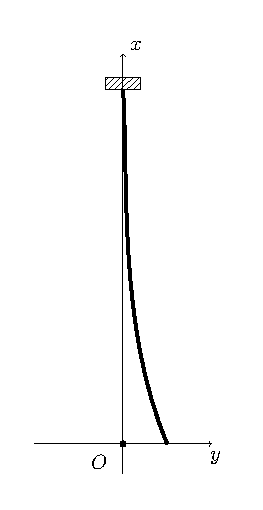
\includegraphics[scale=1]{Imagenes/Cadena_Oscilante_01.eps}
    \caption{Cadena oscilante y el sistema coordenado.}
    \label{fig:figura_cadena_inicial}
\end{figure}

Suponemos que $Y (x, t)$ es pequeña en comparación con la longitud de la cadena $L$. Por lo tanto, no consideramos  la diferencia entre las distancias medidas a lo largo de la cadena y las distancias medidas a lo largo del eje $x$, es decir, podemos omitir los términos:
\begin{align*}
\sqrt{x^{2} + Y^{2}} - x \thicksim \dfrac{Y^{2}}{x}
\end{align*}
Por la misma razón, podemos cancelar el desplazamiento vertical debido a las oscilaciones. También suponemos que el ángulo $\alpha (x)$ entre la dirección local de la cadena y el eje $x$ es pequeño, por lo tanto:
\begin{align}
\sin \alpha \approx \tan \alpha = \pdv{Y}{x}
\label{eq:ecuacion_01}
\end{align}

\subsection{Componentes de la fuerza.}

La componente horizontal de la fuerza neta que actúa sobre un segmento de la cadena de longitud $\Delta x$ debido a la tensión interna $T (x)$ es (ver Fig. 2):
\begin{align}
T (x  + \Delta x) \, \pdv{x} Y (x + \Delta x) - T (x) \, \pdv{x} Y (x) \approx \pdv{x} \bigg[ T (x) \, \pdv{Y}{x}  \bigg] \, \Delta x
\label{eq:ecuacion_02}
\end{align}

\begin{figure}[H]
    \centering
    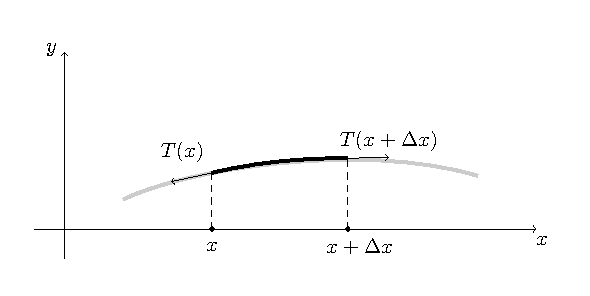
\includegraphics[scale=1.3]{Imagenes/Cadena_Oscilante_02.eps}
    \caption{Fuerzas actuando en el elemento de la cadena.}
    \label{fig:figura_elemento_cadena}
\end{figure}

La segunda ley de Newton nos proporciona la ecuación de movimiento:
\begin{align}
\pdv{x} \bigg[ T (x) \pdv{Y}{x} \bigg] \, \Delta x = \rho \, \Delta x \, \pdv[2]{Y}{x}
\label{eq:ecuacion_03}
\end{align}
donde:
\begin{enumerate}[label=\alph*)]
\item $\rho$ es la densidad lineal de la cadena (masa por unidad de longitud).
\item $\rho \, \Delta x$  es la masa del segmento.
\item $\displaystyle \pdv[2]{Y}{x}$ es la aceleración.
\end{enumerate}

\subsection{Ecuación de movimiento.}

Cancelando el factor común $\Delta x$ en ambos lados de la ec. (\ref{eq:ecuacion_03}), tenemos:
\begin{align}
\pdv{x} \bigg[ T (x) \pdv{Y}{x} \bigg] = \rho \, \pdv[2]{Y}{x}
\label{eq:ecuacion_04}
\end{align}

Para pequeñas oscilaciones de la cadena, cuando podemos cancelar el desplazamiento vertical debido a las oscilaciones, la tensión $T (x)$ es la misma que para la cadena en reposo, es decir, la tensión en el punto con la coordenada vertical $x$ es igual al peso de la parte de la cadena debajo de $x$. Por lo tanto,
\begin{align}
T = \rho \, g \, x
\label{eq:ecuacion_05}
\end{align}
donde $g$ es la aceleración debida a la gravedad.
\par
La cadena está fija en la parte superior, por lo tanto:
\begin{align}
Y (0, t) = 0
\label{eq:ecuacion_06}
\end{align}
El desplazamiento en el extremo libre de la cadena permanece finito en todo momento, así que:
\begin{align}
\abs{Y (L, t)} < \infty
\label{eq:ecuacion_07}
\end{align}

\section{Separación de variables.}

Resolvemos la ecuación diferencial parcial mediante la separación de variables ec. (\ref{eq:ecuacion_03}) con las condiciones de frontera ecs. (\ref{eq:ecuacion_06}), (\ref{eq:ecuacion_07}), es decir, suponiendo que:
\begin{align}
Y (x, t) = y (x) \, u (t)
\label{eq:ecuacion_08}
\end{align}
Sustituyendo la ec. (\ref{eq:ecuacion_08}) en la ec. (\ref{eq:ecuacion_04}), obtenemos:
\begin{align}
u (t) \, \dv{x} \bigg[ T (x) \, \dv{y}{x} \bigg] = \rho \, y (x) \, \dv[2]{u}{t}
\label{eq:ecuacion_09}
\end{align}
que mediante un arreglo de las funciones $u$ e $y$, se tiene:
\begin{align}
\dfrac{1}{y (x)} \, \dv{x} \bigg[ T (x) \, \dv{y}{x} \bigg] = \rho \, \dfrac{1}{u (t)} \, \dv[2]{u}{t}
\label{eq:ecuacion_10}
\end{align}
El lado derecho de la ec. (\ref{eq:ecuacion_10}) es una función del tiempo $t$. El lado izquierdo es una función de $x$. Los dos lados pueden ser iguales en todo momento y coordenadas solo si ambos son iguales a la misma constante.
\par
Como vemos en breve, esta constante debe ser real y negativa. De hecho, el sistema mecánico descrito por la ec. (\ref{eq:ecuacion_03}) es conservativo. Por lo tanto, la función $u (t)$ no puede crecer sin límite o reducirse a cero. Las soluciones permitidas solo son posibles para constantes de separación negativa reales.

\subsection{Sistema de EDO.}

Denotando la constante de separación por $- \omega^{2}$, obtenemos las siguientes ecuaciones:
\begin{align}
\dfrac{1}{u (t)} \, \dv[2]{u}{t} &= - \omega^{2} \label{eq:ecuacion_11} \\[0.5em]
\dfrac{1}{y (x)} \, \dv{x} \bigg[ T (x) \, \dv{y}{x} \bigg] &= - \rho \, \omega^{2} \label{eq:ecuacion_12}
\end{align}
La ec. (\ref{eq:ecuacion_11}) se resuelve fácilmente:
\begin{align}
\dv[2]{t} + \omega^{2} \, u (t) = 0
\label{eq:ecuacion_13}
\end{align}
cuya solución es del tipo:
\begin{align}
u (t) = A \, \cos (\omega t) + B \, \sin (\omega t)
\label{eq:ecuacion_14}
\end{align}
donde $A$ y $B$ son constantes de integración reales. Vemos que $\omega$ es la frecuencia de las oscilaciones de la cadena.
\par
La ecuación para la amplitud de las oscilaciones, $y (x)$, es:
\begin{align}
\dv{x} \bigg[ T (x) \, \dv{y}{x} \bigg] = - \rho \, \omega^{2} \, y (x)
\label{eq:ecuacion_15}
\end{align}
Usando la expresión para la tensión en la cadena, ec. (\ref{eq:ecuacion_05}), se tiene que:
\begin{align}
\dv{x} \bigg[ x \, \dv{y}{x} \bigg] + \dfrac{\omega^{2}}{g} \, y(x) = 0
\label{eq:ecuacion_16}
\end{align}

Las condiciones de frontera para la ec. (\ref{eq:ecuacion_16}) son:
\begin{align}
y (L) = 0 \hspace{1.5cm} \abs{y (0)} < \infty
\label{eq:ecuacion_17}
\end{align}

Para resolver la ec. (\ref{eq:ecuacion_16}) hagamos el cambio de variable $x \to z$:
\begin{align}
z = 2 \sqrt{\dfrac{\omega^{2}}{g} \, x}
\label{eq:ecuacion_18}
\end{align}
por lo tanto:
\begin{align}
\begin{aligned}[b]
\dv{z}{x} &= \sqrt{\dfrac{\omega^{2}}{g x}} \\[0.5em]
\dv{y}{x} &= \dv{y}{z} \, \dv{z}{x} = \sqrt{\dfrac{\omega^{2}}{g x}} \, \dv{y}{z} \\[0.5em]
\Rightarrow \hspace{0.2cm} x \, \dv{y}{x} &= \sqrt{\dfrac{\omega^{2}}{g} \, x} \, \dv{y}{z} = \dfrac{z}{2} \, \dv{y}{z}
\end{aligned}
\label{eq:ecuacion_19}
\end{align}
por lo que:
\begin{align}
\dv{x} \bigg[x \, \dv{y}{x} \bigg] = \dv{z} \bigg[ \dfrac{z}{2} \, \dv{y}{z} \bigg] = \dfrac{1}{2} \, \sqrt{\dfrac{\omega^{2}}{g x}} \, \dv{z} \bigg( z \, \dv{y}{z} \bigg)
\label{eq:ecuacion_20}
\end{align}

La ecuación de movimiento ec. (\ref{eq:ecuacion_16}) cambia a la expresión:
\begin{align}
\dfrac{1}{2} \sqrt{\dfrac{\omega^{2}}{g x}} \, \dv{z} \bigg( z \, \dv{y}{z} \bigg) + \dfrac{\omega^{2}}{g} \, y = 0
\label{eq:ecuacion_21}
\end{align}
que de manera equivalente es:
\begin{align}
\dv{z} \bigg( z \, \dv{y}{z} \bigg) + z \, y = 0
\label{eq:ecuacion_22}
\end{align}
Al expandir la derivada, se obtiene:
\begin{align}
z \, \dv[2]{y}{z} + \dv{y}{z} + z \, y = 0
\label{eq:ecuacion_23}
\end{align}

\subsection{Ecuación de Bessel de orden cero.}

La ec. (\ref{eq:ecuacion_23}) es una ecuación de Bessel de orden cero. La solución general es de la forma:
\begin{align*}
y (x) = A \, J_{0} (z) + B \, Y_{0} (z)
\end{align*}
Recordemos que $Y_{0} (z) \to \infty$ cuando $z \to 0$, por lo que la constante $B$ debe de ser tal que $B = 0$, por lo que la solución satisface las condiciones de frontera ec. (\ref{eq:ecuacion_17}):
\begin{align}
y (x) = J_{0} (z) = J_{0} \bigg( 2 \omega \sqrt{\dfrac{x}{g}} \bigg)
\label{eq:ecuacion_24}
\end{align}
La condición en el extremo de la cadena que está fijo es $y (L) = 0$, lo que determina las frecuencias características de la cadena:
\begin{align}
J_{0} \bigg( 2 \, \omega \, \sqrt{\dfrac{L}{g}} \bigg) &= 0 \label{eq:ecuacion_25} \\[0.5em]
\omega_{n} &= \dfrac{1}{2} \, \sqrt{\dfrac{g}{L}} \, z_{n} \label{eq:ecuacion_26}
\end{align}
donde los $z_{n}$ son las raíces de la función de Bessel $J_{0} (x)$.

\subsection{Raíces de \texorpdfstring{$J_{0} (x)$}{J0 (x)}.}

En la tabla (\ref{table_Tabla_Ceros_J0}) se presentan las primeras raíces, mientras que en la figura (\ref{fig:figura_raices_J0}) se presenta la gráfica de $J_{0} (x)$ con los valores que son raíces.
\begin{table}[H]
\centering
\large
\begin{tabular}{c | l}
$k$ & $z_{k}$ \\ \hline
$1$ & $2.40483$ \\
$2$ & $5.52008$ \\
$3$ & $8.65373$ \\
$4$ & $11.7915$ \\
$5$ & $14.9309$ \\
\end{tabular}
\caption{Raíces de la función $J_{0} (x)$.}
\label{table_Tabla_Ceros_J0}
\end{table}
Los modos normales de la cadena colgante son:
\begin{align}
y_{n} (x) = J_{0} \bigg( z_{n} \, \sqrt{\dfrac{x}{L}} \bigg)
\label{eq:ecuacion_28}
\end{align}

\begin{figure}[H]
    \centering
    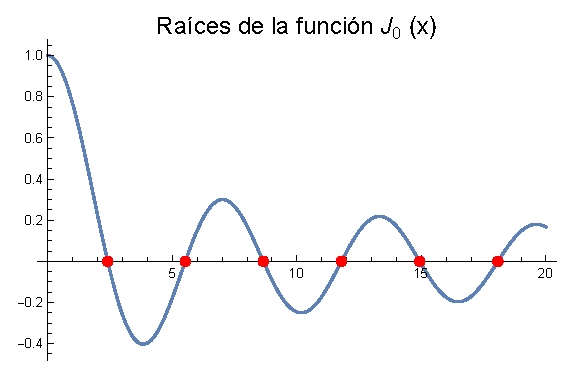
\includegraphics[scale=1.2]{Imagenes/Plot_Bessel_Cadena_01_Raices_J0.eps}
    \caption{Gráfica de $J_{0}$ y sus raíces.}
    \label{fig:figura_raices_J0}
\end{figure}

En las figuras (\ref{fig:figura_modo_z1}), (\ref{fig:figura_modo_z2}) y (\ref{fig:figura_modo_z3}) se presenta un esquema del modo de oscilación de la cadena colgante, con las raíces $z_{1}$, $z_{2}$ y $z_{3}$, respectivamente.
\begin{figure}[H]
    \centering
    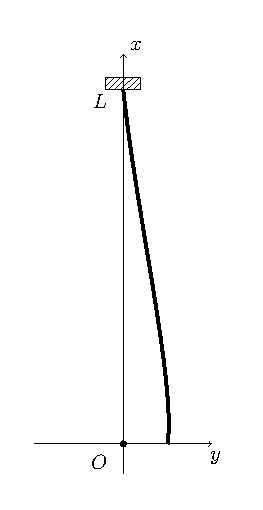
\includegraphics[scale=1]{Imagenes/Cadena_Oscilante_03.eps}
    \caption{Modo de oscilación de la cadena con $z_{1}$.}
    \label{fig:figura_modo_z1}
\end{figure}
\begin{figure}[H]
    \centering
    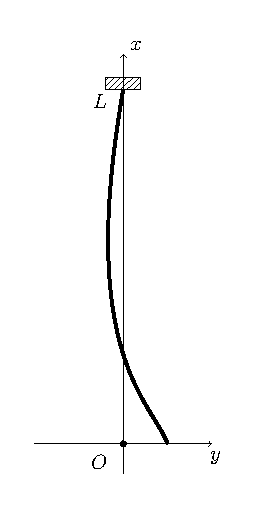
\includegraphics[scale=1]{Imagenes/Cadena_Oscilante_04.eps}
    \caption{Modo de oscilación de la cadena con $z_{2}$.}
    \label{fig:figura_modo_z2}
\end{figure}
\begin{figure}[H]
    \centering
    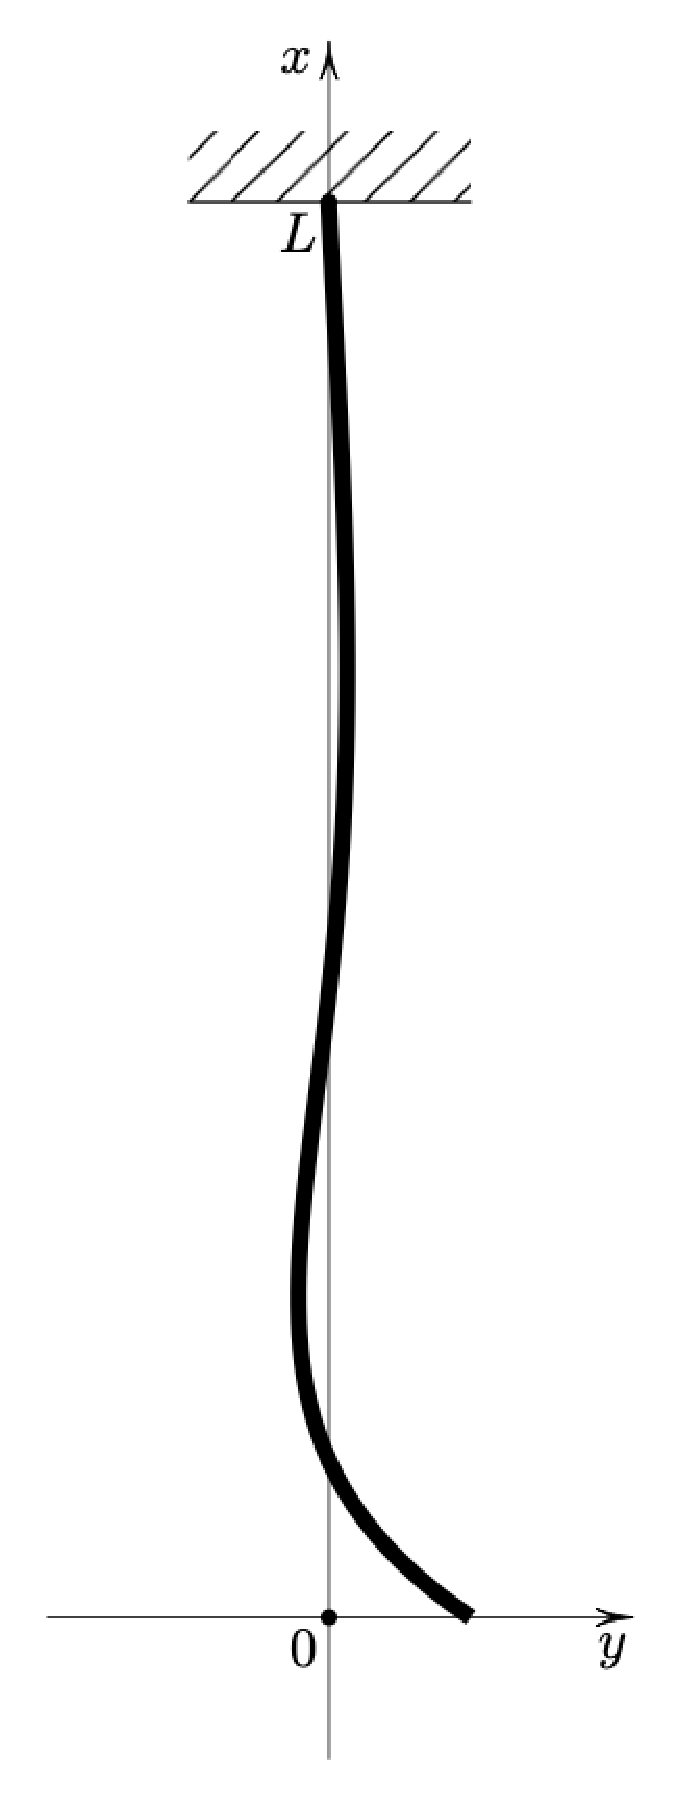
\includegraphics[scale=0.3]{Imagenes/Cadena_Oscilante_05_png.eps}
    \caption{Modo de oscilación de la cadena con $z_{3}$.}
    \label{fig:figura_modo_z3}
\end{figure}

\end{document}